%==============================================================================
%== template for LATEX poster =================================================
%==============================================================================
%
%--A0 beamer slide-------------------------------------------------------------
\documentclass[final]{beamer}
\usepackage[orientation=portrait,size=a0,
            scale=1.35        % font scale factor
           ]{beamerposter}
           
\geometry{
  hmargin=2.5cm, % little modification of margins
}

%
\usepackage[utf8]{inputenc}
\graphicspath{{./img/}}
\linespread{1.15}
%
%==The poster style============================================================
\usetheme{sharelatex}

%==Title, date and authors of the poster=======================================
\title
[Super Conference, 1 - 10 July 2013, New York, USA] % Conference
{ % Poster title
{\huge Learning Hand-Eye Coordination for a Humanoid Robot using SOMs}
}

\author{ % Authors
Ivana Kaji\'c\inst{1}, Guido Schillaci\inst{2}, Sa\v{s}a Bodiro\v{z}a\inst{2}, Verena V. Hafner\inst{2}
}
\institute
[Very Large University] % General University
{
\inst{1} Bernstein Center for Computational Neuroscience Berlin, Berlin, Germany\\[0.3ex]
\inst{2} Cognitive Robotics Group, Department of Computer Science, Humboldt-Universit\"at zu Berlin, Germany
}
\date{\today}



\begin{document}
\begin{frame}[t]
%==============================================================================
\begin{multicols}{2}
%==============================================================================
%==The poster content==========================================================
%==============================================================================
%\hspace{-1cm}
\section{Introduction}

Acquisition of hand-eye coordination skills is a prerequisite for more complex behaviors used in social interactions. Pointing gestures are often employed to steer the attention of participants and are thus an integral part of spontaneously flowing human-robot interaction. We propose a biologically inspired model and implement it on a humanoid robot to analyze pointing \cite{Kaplan}.
%The onset of pointing behavior in infants still remains an open question \cite{Kaplan}. 
%We addressed that question by proposing a biologically inspired model implemented on a humanoid robot. 
The model is based on self-organizing maps (SOMs) and the Hebbian learning paradigm. In the experiment we showed that the robot equipped with such a model exhibits pointing when an object is presented out of reach of its hand. 

\section{Random Motor Babbling}

%Self-exploration mechanism is one of the most basic learning behaviors in humans.
Motor babbling is a \emp{self-exploration} mechanism for acquiring sensorimotor experience.
An adapted random motor babbling algorithm \cite{Schillaci} was implemented on a \emp{humanoid robot} Nao for learning of left arm postures. 
%The robot learned \emp{left arm postures} in terms of 3D hand coordinates and 4D joint (2D shoulder and 2D elbow) coordinates. %In total, the 40 minutes long babbling procedure yielded 74,143 7D vectors that were used for the training of the model.

\vskip2ex
\begin{figure}[t!]
\centering
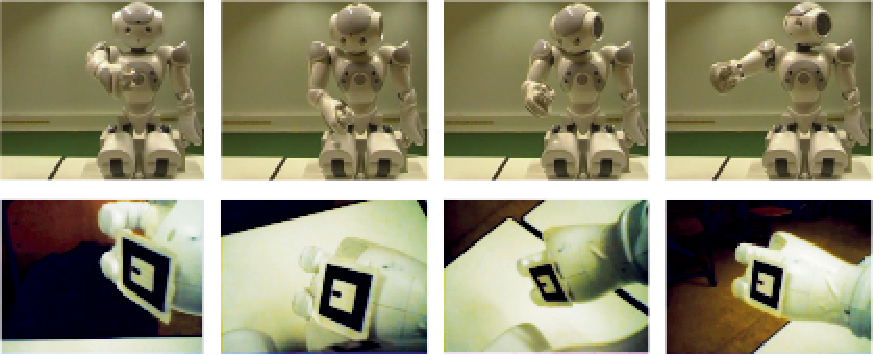
\includegraphics[width=0.99\columnwidth]{sequence}
\caption{Random motor babbling sequence in a robot}
\end{figure}
\vskip2ex


\section{The Model}

\subsection{Description}
The model is inspired by \emp{topographic maps} observed in the sensorimotor areas of the cortex. It consists of \emp{two associated 2D SOMs} (Figure \ref{fig:model}).

%with an equal number of neurons arranged in rows and columns. 
%Neurons in the first SOM were identified as 3D weight vectors and neurons in the second SOM as 4D weight vectors. 
Two different instances of a model were trained to simulate two different stages of skill development:  the \emp{$5\times 5$ model} and the \emp{$15\times 15$ model}. %The latter model simulates a more advanced stage of skill development that is characterized by a greater number of specialized neurons. %Models were given names based on the number of neurons in rows and columns in an SOM.
%Names of the models stem from the number of neurons in rows and columns in an SOM.


\subsection{Training}
The training comprised of following steps:

\begin{enumerate}
 \item Presentation of the 3D hand coordinates to the first SOM and 4D joint coordinates to the second SOM
 \item Identification of \emp{winning neurons} in both SOMs 
 \item Strengthening of \emp{Hebbian connections} between the two winning neurons
\end{enumerate}

\begin{beamercolorbox}[wd=1\linewidth,colsep=0.03cm]{colorbar}
\end{beamercolorbox}

\subsubsection{Acknowledgments}
{\small  
This work has been supported by the Bernstein Center for Computational Neuroscience Berlin and by the EU-funded ITN INTRO (INTeractive RObotics research network).}

\subsubsection{References}
\bibliographystyle{abbrv}
% \bibliography{references}
\begin{thebibliography}{99}

\bibitem{Kaplan} F. Kaplan and V. V. Hafner. The challenges of joint attention., Interaction Studies, 7(2):135–169, 2006.

% \bibitem{Kohonen} T. Kohonen.
% Neurocomputing: Foundations of research.
% chapter Self-organized Formation of Topologically Correct Feature Maps, pages 509–521. MIT Press, Cambridge, MA, USA, 1988.

\bibitem{Schillaci} G. Schillaci and V. V. Hafner. Random movement strategies in self-exploration for a humanoid robot. In A. Billard, P. H. K. Jr., J. A. Adams, and J. G. Trafton, editors, HRI, pages 245–246. ACM, 2011.

\bibitem{Morse} A. Morse, J. de Greeff, T. Belpaeme, and A. Cangelosi. Epigenetic robotics architecture (era).
Autonomous Mental Development, IEEE Transactions on, 2(4):325–339, 2010.

\end{thebibliography}



\newpage
\begin{figure}[h]
\centering
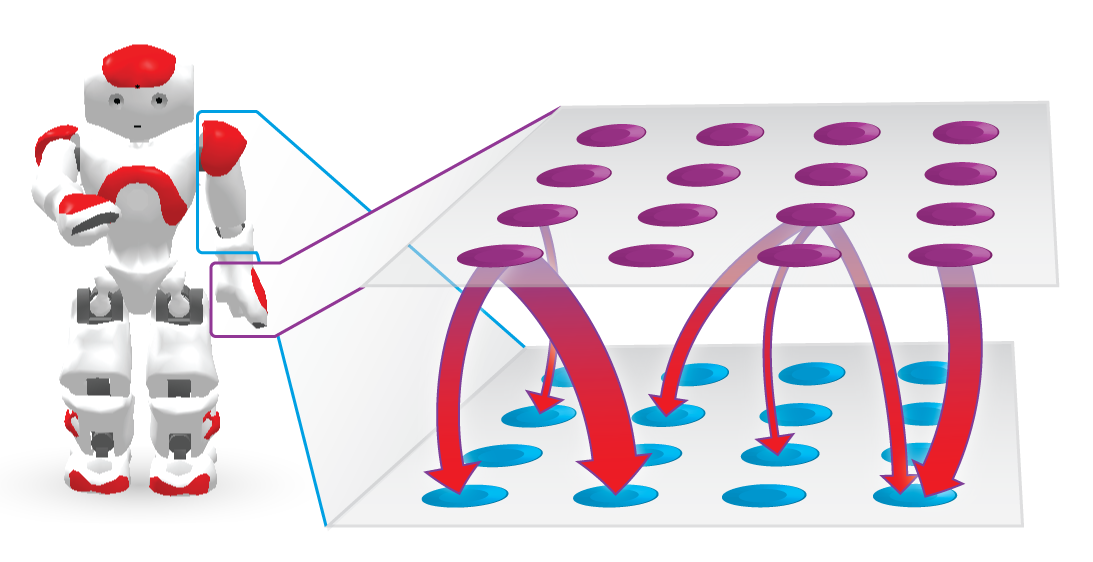
\includegraphics[width=0.9\columnwidth]{model.png}
\caption{The SOM-based model}
\label{fig:model}
\end{figure}
%\vskip1ex


% Neural weights ($\mathbf{w}$) in SOMs were iteratively adjusted using the following learning rule:
% $$
% \mathbf{\Delta w_{j}} = \eta_s(t) h(i, j) (\mathbf{w_{j}}-\mathbf{x_p})
% $$
% 
% Weights linking the two winning neurons in SOMs were adjusted using a positive Hebbian learning rule:
% $$
% \Delta w_{ij} = \eta_h A_i(\mathbf{x}) A_j(\mathbf{y})
% $$

\vspace{-2.4cm}
\section{The Experiment and Results}
A human subject was holding and randomly moving an object tagged with a marker in front of the robot for approximately 2.5 minutes. The robot followed the object with its head and arm. The robot pointed to the object if it was presented out of its reach (Figure \ref{fig:experiment}). 

\vskip2ex
\begin{figure}[t!]
\centering
\includegraphics[width=0.99\columnwidth]{double_thick.png}
\caption{SOM with 225 neurons covering the left hand babbling trajectory (a),  hand and object positions from the experiment (b)}
\label{fig:double}
\end{figure}
\vskip2ex

Compared to the $5 \times 5$ model ($Mean\ error=99.93mm$
, $Std.\ Dev.=32.10$), there was a significant \emp{improvement in pointing} accuracies for the $15 \times 15$ model ($Mean\ error=80.32mm$, $Std.\ Dev.=33.41$), conditions; $t(1400)=76.47$, $p<0.05$.

\vskip1ex
\begin{figure}[t!]
\centering
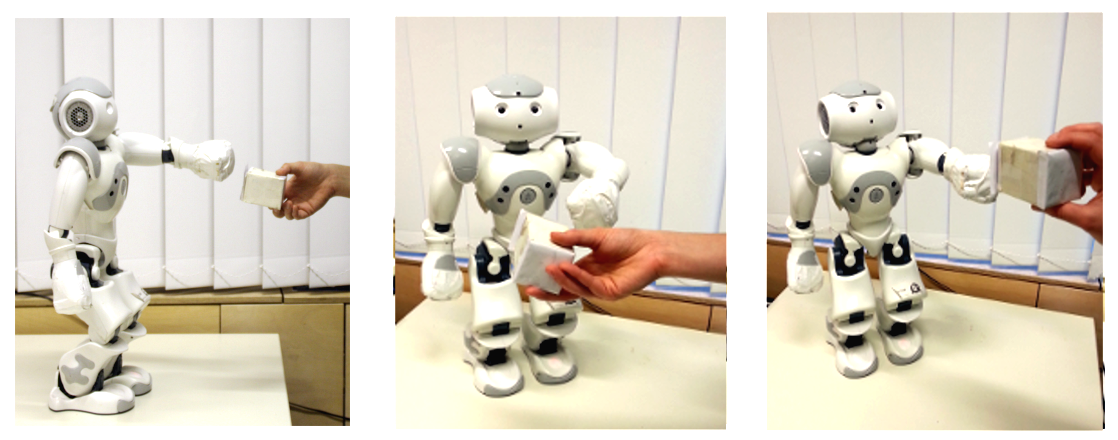
\includegraphics[width=0.99\columnwidth]{experiment_new.png}
\caption{The experiment. The robot points to the tagged object}
\label{fig:experiment}
\end{figure}
%\vskip1ex
\vspace{-1.5cm}
\section{Conclusion}
The SOM-based model explains how pointing behavior emerges from sensorimotor learning of hand-eye coordination. The experiment demonstrates that a humanoid robot equipped with the model exhibits pointing through body babbling. An increase in the size of the SOMs improves the accuracy of pointing. 

%\vspace{-.8cm}

%==============================================================================
%==End of content==============================================================
%==============================================================================

%--References------------------------------------------------------------------
\vspace{-1cm}

%--End of references-----------------------------------------------------------

\end{multicols}

%==============================================================================
\end{frame}
\end{document}
